%\chapter{Introduction}
%\textit{by Olaf Kolditz and Hua Shao}

Coupled process modelling has been already considered in the various engineering problems and geo-scientific applications as the computation method was introduced for problems of soil consolidation and dam construction, and oil/gas filed exploration since early 1970. However, substantial progress in experimental and theoretical studies regarding the fully coupling effects of temperature, hydraulics, mechanics, as well as chemistry in fractured porous media was just made in the last two decades due mainly to demands from the performance and safety assessment of a high-level nuclear waste repository. Numerical methods and computer codes have been developed successfully within the international DECOVALEX project (1992 - 2011). Meanwhile a wider range of applications associated with THMC coupled problem such geothermal reservoir engineering, CO2-storage, construction of underground opening etc. can be found in the different international conferences, e.g. GeoProc (www.mech.uwa.edu.au/research/geoproc), ComGeo (www.com-geo.org/).

For a long-term performance and safety assessment of a nuclear waste repository in deep geological formation, an important issue is the impact to guarantee the isolation of an underground repository. To answer this question, solute transport process under the coupled conditions involving mechanical stability, thermal loading from the high-level waste, and chemistry in the groundwater should be predicted numerically. Also, for the construction planning of such complex and implementation of experimental data gained from the in situ tests a multiple process coupled code is required. 

In the course of the quick development of computer technology, complicated geoscientific and geotechnical problems can be analysed in a coupled manner using modern numerical codes.
However, the understanding of the complicated coupled processes based on the experimental data available and implementation of the developed algorithm into the numerical codes are major challenge for the scientists, which require an interdisciplinary cooperation and interactive procedure. 

Quality management is nowadays a standard tool for production and development to ensure a high quality of a produced result. A numerical code dealing with the coupled THMC process is highly complicated software product, since the different processes have different characteristic features, e.g. time and spatial scales, nonlinearities, and interaction degree etc.. To keep the high quality of the developed code, benchmark testing is therefore necessary, especially in case scientists from different disciplinary and different organisation are working on the same code. Therefore, code verification and validation of selected test case are documented during the code development, and finally a benchmarking book for code developer (DBB) is produced and quality ensured.
%-------------------------------------------------------------------------
\subsection*{Scope of this book}

The intention of this book is multifold and can be summarised as follow:
\begin{compactitem}
  \item Outline the theoretical background of THMC processes in porous media for applications in geotechnics and hydrology (Part I),
  \item Provide collected test cases which can be used for benchmarking the numerical code development for single (Part II) as well as coupled processes (Part III),
  \item Help to develop and set-up applications (www.opengeosys.net and connected OpenGeoSys development platform available through the internet, see also Appendix for more details)
\end{compactitem}

%-------------------------------------------------------------------------
\subsection*{Application areas}

\subsubsection{Geotechnics}

The coupling phenomena of thermal (T), hydraulic (H), and mechanical (M) processes are important for the analysis of deep geosystems under high temperature, pressure and stress conditions. Application areas of THM coupled models are e.g. geothermal energy utilization, nuclear waste disposal, and carbon dioxide storage in the deep geological formation.

The following slides illustrate that the understanding of THM processes including chemical reactions (C process) is important to a large variety geotechnical and geothermal applications. The physical basics are exactly the same for these applications. Different is simply

\begin{compactitem}
	\item the geological environment and different rock types, i.e. crystalline rocks, volcanic rocks, sandstones, clay, bentonite, ...
	\item the geofluids, i.e. water, brines, vapour, methane, carbon dioxide ...
	\item the thermodynamic conditions, i.e. temperature, stress, pressure, salinity, ...
\end{compactitem}

\begin{figure}[!htb]
\begin{minipage}[t]{0.48\textwidth}
Fig. \ref{fig:apl1} shows the application area: nuclear waste disposal in deep geological formations.
There are several concepts concerning host rock for the disposal of hazardous waste in deep geological media, i.e. crystalline, salt, sediment, and volcanic formations. Different concepts use different buffer systems as geotechnical barrier for the waste isolation, i.e. crushed salt, bentonite, and bentonite/sand mixture. THM/C coupled modelling is required for the long-term analysis of possible processes which might result in a release of contaminants from the repository \cite{NowakEtAl:2011}. In that case it is important to know, how long it will take until the contaminants can return into the biosphere.
\end{minipage}
\hspace{0.02\textwidth}
\begin{minipage}[t]{0.48\textwidth}
%\vspace{3.5cm}
\vspace{1.5cm}
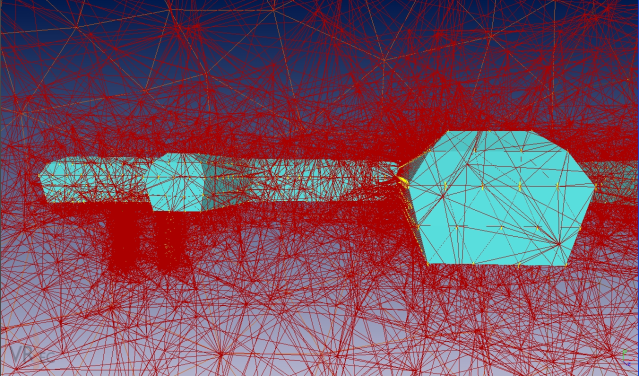
\includegraphics[scale=0.25]{figures/intro1}
\caption{Tunnel system (Visualization by B. Zehner)}
\label{fig:apl1}
\end{minipage}
\end{figure}

\vspace{-3cm}

\begin{figure}[!htb]
\begin{minipage}[t]{0.48\textwidth}
Fig. \ref{fig:apl2} illustrates the application area: Carbon Capture Storage (CCS). The idea is to capture the \CO2 from the power plants, liquefy it and inject it into the subsurface for long-term storage. Two basic concepts for appropriate geological systems are under proof now: depleted gas reservoirs and deep saline aquifers. After many years of operation many former gas reservoirs are depleted. These reservoirs are in an underpressurized status and can take up large volumes of fluids. Keeping the reservoir underpressurized and the impervious cap rocks are part of the storage concepts. THM/C modelling is required in order to calculate the possible fluid storage capacity and to better understand the highly coupled processes in the \CO2 injection area as well as their consequences for the storage concept \cite{GorkeEtAl:2011}.
\end{minipage}
\hspace{0.02\textwidth}
\begin{minipage}[t]{0.48\textwidth}
%\vspace{5cm}
\vspace{2cm}
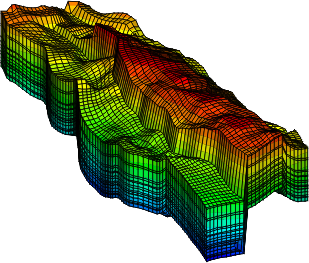
\includegraphics[scale=0.5]{figures/intro2}
\caption{Subsurface reservoir for CO2 storage}
\label{fig:apl2}
\end{minipage}
\end{figure}

\newpage

\begin{figure}[!htb]
\begin{minipage}[t]{0.48\textwidth}
Fig. \ref{fig:apl3} depicts the application area: Geothermal energy, which is one of the alternative future energy resources under consideration. So-called shallow and deep geothermal systems are distinguished. Shallow systems are already commercially used e.g. for heating purposes. Deep geothermal reservoirs can be used for electric power production as high temperatures up to 200 C can be produced. THM/C modeling is required to design those geothermal power plants, e.g. in order to optimize production efficiency and reservoir lifetime. The significant cooling of the reservoir due to fluid reinjection gives raise to thermo-mechanical effects which needs to be controlled in order to avoid reservoir damage \cite{WatanabeEtAl:2010}.
\end{minipage}
\hspace{0.02\textwidth}
\begin{minipage}[t]{0.48\textwidth}
%\vspace{4cm}
\vspace{1cm}
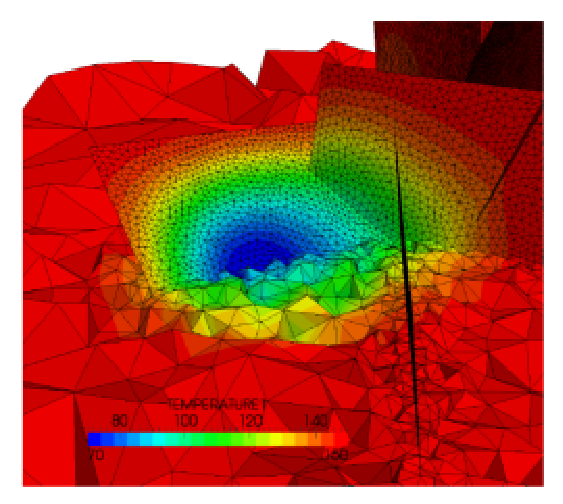
\includegraphics[scale=0.63]{figures/intro3}
\caption{Simulated temperature field of water reinjection}
\label{fig:apl3}
\end{minipage}
\end{figure}

%-------------------------------------------------------------------------

\begin{figure}[!htb]
\begin{minipage}[t]{0.48\textwidth}
\subsubsection{Hydrology}

The second application area for coupled process simulation is hydrology. River basins or catchments are also subject to THMC coupled processes, of course in a completely different range of thermodynamic conditions as deep geological systems. Hydrological processes are very complex to describe as they vary highly in time and in space.
The evaluation of groundwater recharge is most important to a sustainable water resources management (so called safe yield).
To this purpose, i.e. the understanding of small scale phenomena such as root / soil water interaction is of tremendous significance \cite{KalEtAl2010}.
Typically groundwater models are used for management purposes particularly in semi-arid areas as the Jordan Valley in the Middle East \cite{WuEtAl:2011}.
\end{minipage}
\hspace{0.02\textwidth}
\begin{minipage}[t]{0.48\textwidth}
%\vspace{6cm}
\vspace{1cm}
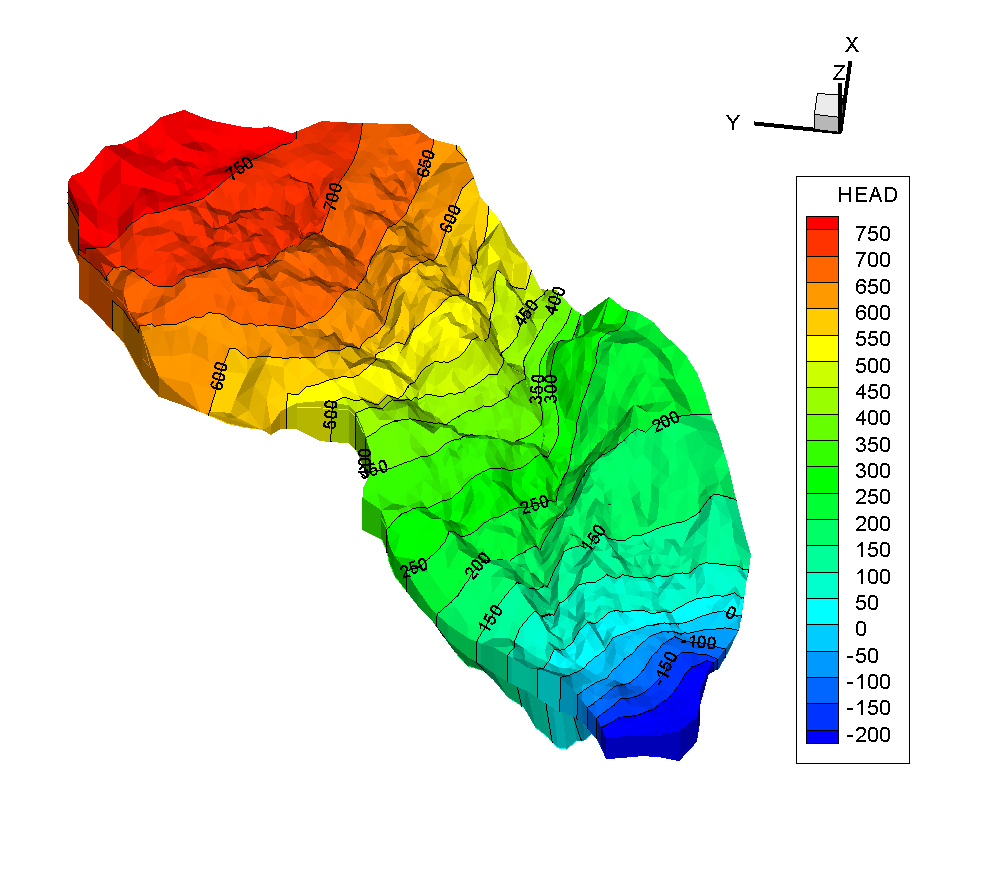
\includegraphics[scale=0.18]{figures/Steady_ContourMap}
\caption{Groundwater model for the Wadi Kafrein catchment in Jordan}
\label{fig:apl4}
\end{minipage}
\end{figure}

\begin{figure}[!htb]
\begin{minipage}[t]{0.48\textwidth}
As water availability is an important issue in semi-arid and arid regions, groundwater quality is deteriorated in many urban areas of the world.
Fig. \ref{fig:apl5} shows as an example a part of a groundwater quality model prepared for the Nankou basin in greater Beijing area.
The idea of this modelling project is to identify possible sources for nitrate contamination originating from intense agriculture and fertilizer production \cite{SunEtAl2010}. Land use and climate changes will impact the availability and quality of water resources to a large degree in the future. The modelling should help to develop scenarios for improving the groundwater quality in the long term. Areas subject to large groundwater abstraction are also endangered to severe land subsidence.
\end{minipage}
\hspace{0.02\textwidth}
\begin{minipage}[t]{0.48\textwidth}
\vspace{2cm}
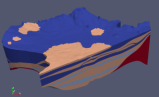
\includegraphics[scale=1]{figures/intro4}
\caption{Nankou groundwater quality model \cite{SunEtAl2010}}
\label{fig:apl5}
\end{minipage}
\end{figure}

%-------------------------------------------------------------------------

\begin{figure}[!htb]
\begin{minipage}[t]{0.48\textwidth}
\subsection{Energy storage}

A very recent research area for THMC modelling became energy storage. The economy and feasibility of renewable energy sources will depend on a large degree on efficient energy storage systems. Fig. \ref{fig:apl6} shows the numerical simulation of flow and heat distribution in a solid thermal energy storage block which will be used to store solar energy collected during days for use at nights (so called solar-thermics). The long term stability and efficiency of those energy storage devices can be optimized using THMC modelling (i.e. solving the inverse geothermal problem). In addition to thermal storage, thermo-chemical concepts are under development, i.e. storing thermal energy by triggering endothermic reactions and gaining thermal energy back on demand with the reverse reaction (exothermic).
\end{minipage}
\hspace{0.02\textwidth}
\begin{minipage}[t]{0.48\textwidth}
%\vspace{4.5cm}
\vspace{1.5cm}
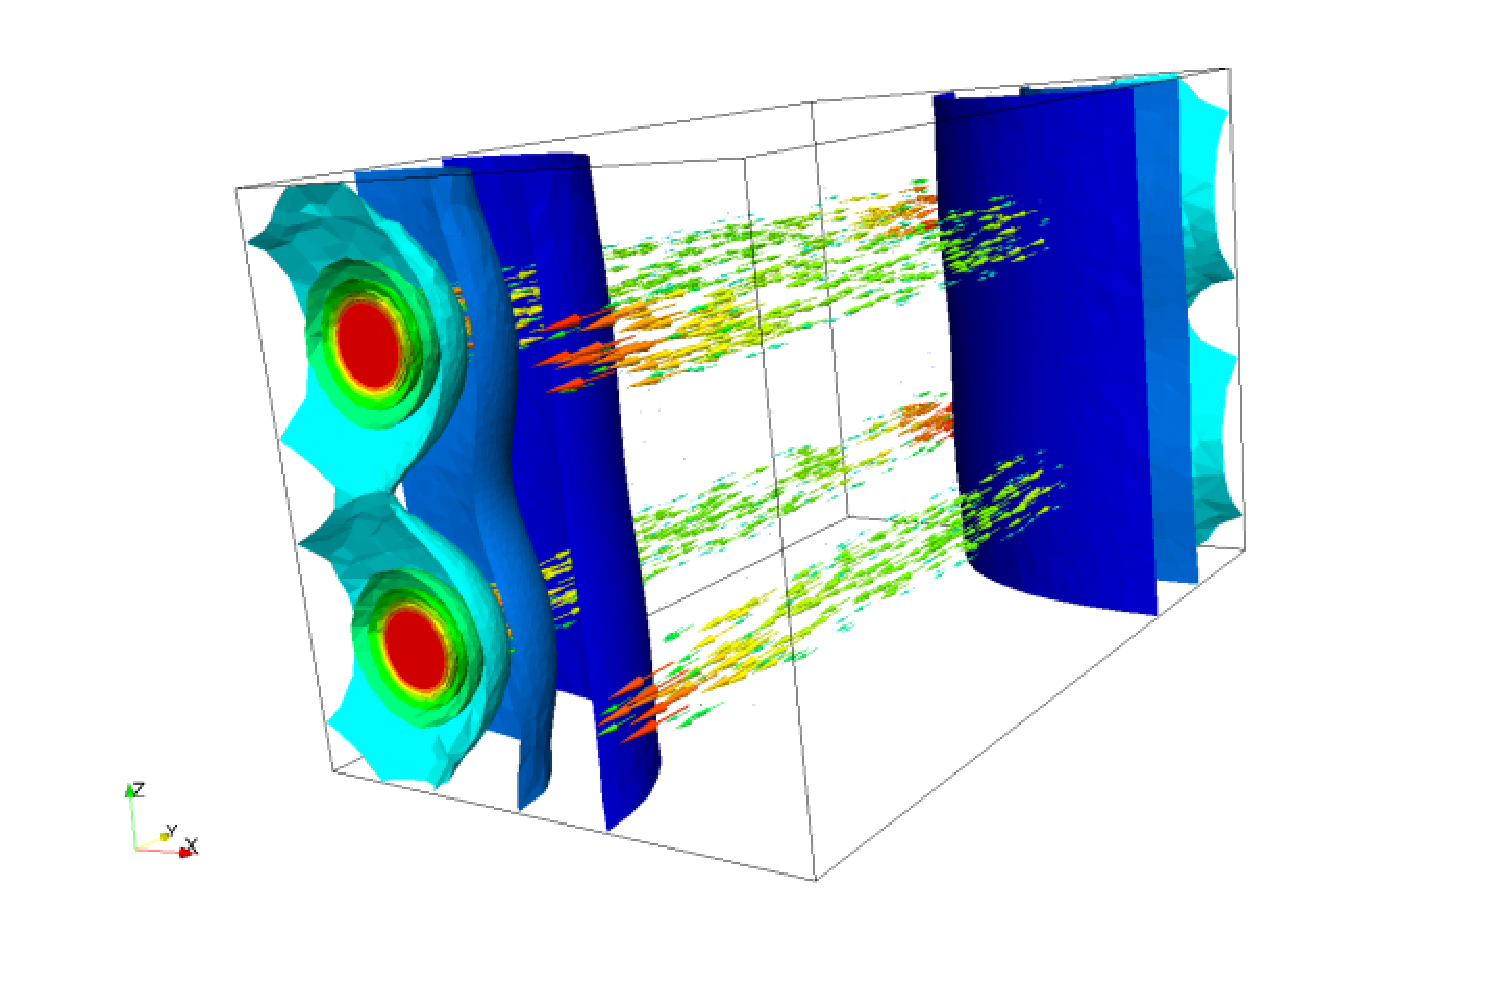
\includegraphics[scale=0.3]{figures/intro5}
\caption{Optimizing energy storage concepts by modelling (OGS simulation by Wenqing Wang), \cite{HGFEnergy:2010}}
\label{fig:apl6}
\end{minipage}
\end{figure}
